%--------------------------------------------------------------------------------------------------------------
% kapitel/grundlagen.tex
%--------------------------------------------------------------------------------------------------------------

\chapter{Grundlagen}
\section{Unterkapitel}
In dem ersten Kapitel sind die Grundlagen der Arbeit darzustellen. Auf Beweise und ausführliche Herleitungen kann verzichtet werden, soweit diese in der Literatur bekannt sind.
Umfangreichere Zwischenrechnungen und eigene Herleitungen sollten im Anhang untergebracht werden.

\subsection{Bilder}
Beispiel für ein Bild in \LaTeX{}
\begin{figure}[ht]
	\begin{center}
		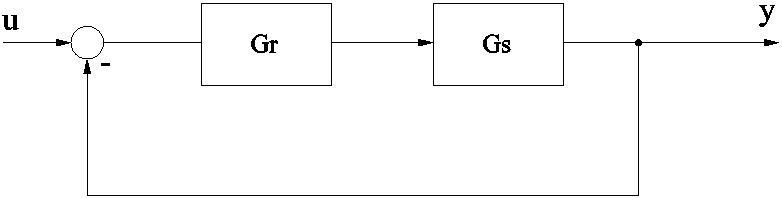
\includegraphics[scale=0.3]{bilder/regelkreis.png}
		\caption{Ein Standard-Regelkreis}
		\label{pic:grund:regelkreis}
	\end{center}
\end{figure}

\subsection{Tabellen}
Beispiel für eine Tabelle in \LaTeX{}
\begin{table}[ht]
	\begin{center}
		\caption{Verwendete Matrizen}
		\begin{tabular}{|l|l|l|}
			\hline
			Matrix& Dimension& Symbol\\
			\hline
			Systemmatrix& $n\times n$& \textrm{A}\\
			\hline
			Ausgangsmatrix& $m\times n$& \textrm{C}\\
			\hline
		\end{tabular}
		\label{tab:grund:matrizen}
	\end{center}
\end{table}

\subsection{Formeln}
Beispiel für eine Formel in \LaTeX{}
\begin{equation}
	c^2 = a^2 + b^2
\end{equation}
und noch eine Formel
\begin{equation}
	f_1(x) = x_1 + x_2 + x_3
\end{equation}
Für weitere Möglichkeiten Formeln in \LaTeX{} einzufügen, schauen sie bitte in \cite{Peters2005}.

\subsection{{Bib\TeX}}
Bib\TeX{} ermöglicht das erstellen eines Literaturverzeichnisses. Für die die sich weiter einarbeiten wollen, empfehle ich folgende Seite \cite{wiki:bibtex}.

\subsection{Abkürzungen}
Es wird das Package \textit{glossary} verwendet. Mit ihm ist es möglich ein Abkürzungsverzeichnis und ein Glossary zu erstellen. Beispiel: \acrfull{lan} \acrfull{www}
